\newpage
\section{The Latitude DPOS Consensus Algorithm}
\label{app:dpos}

Latitude uses the Delegated Proof of Stake algorithm for consensus. This method allows honest participants and stake
holders to partake in block production. The same philosophy is also used for electing the Governance council. All
operations are transparent and any participant can become part of such operations through honest commitment to the
system.

Like other PoS chains, DPoS doesn’t include miners who run hashes to produce blocks . Instead, an elected subset of
participants is chosen to perform the work of validating the chain. These participants are called block producers,
delegates, notaries, validators, forgers, or witnesses. DPOS or variants thereof is being widely used in the blockchain
space, current blockchains utilizing DPoS include:

\begin{itemize}
\item EOS, BitShares, Steem, Golos, Ark, Lisk, PeerPlays, Nano (formerly Raiblocks), and Tezos
\item Cosmos/Tendermint, Cardano, and a few others use consensus algorithms loosely based on DPoS
\end{itemize}

Latitude uses a combination of stake (amount of LAT token held as collateral) and trust (value in the trust ledger as
discussed in Section \ref{sec:trust}. The block production algorithm works as follows:

\begin{itemize}
\item Participants who own a certain amount of trust and stake are allowed to act as delegates. Trust and stake are
    combined into a single metric called the l-factor as given in Equation \ref{eq_l_factor}.
\item Delegates can choose to nominate block producers. Their vote is weighted by their l-factor value. The block
    candidates who receive the most votes are elected to be block producers. Users can also delegate their voting power
        to others on their behalf. Thus DPOS creates a representative democracy with stake and trust based suffrage.
\item The number of block producers is lower bounded $N_{min}$ and upper bounded $N_{max}$, but is not a strict value.

\item Block producers can be voted out any time if bad behavior is determined. The threat of loss of stake and/or
    reputation is a deterren to bad behavior. Also slashing conditions can be easily implemented if so desired.
\item Block consensus: Once a block producer set is determined, a consensus algorithm such as PBFT is used to
    achieve $2/3 +1$ majority to decide on a block. Producers always converge to the longest chain as as long as a
        majority of the block producers are honest, the system will converge.
\item Block production time: This can be set to a desirable value, such as 0.5 or 1 second to make it periodic.
\end{itemize}

DPoS doesn’t attempt to “find” a balance between the number of block producers needed to ensure that control is
sufficiently decentralized and the number of block producers that can easily be monitored for bad behavior. Rather, it
explicitly sets the balance, though it can be modified later through governance protocols.

\noindent
{\em Rewards for block production:} While some blockchains such as EOS, purely reward block producers through inflationary
economics, Latitude uses a combination of trasaction rewards and inflation. The rewards allow nodes that demonstrate
trust (and less stake) to earn tokens. The exact distribution of reward vs inflation based earnings shall be determined
via experiments and research on the testnet.

\noindent
{\em Scalability of the consensus algorithm:}

\newpage
\section{Scaling the Latitude Architecture}
\label{app:latchain}

As the Latitude platform grows both in terms of aggregate data/users or partners, it might become necessary to split
each application vertical into its own side-chain. A Latitude base-chain will work with various side-chains to enforce
basic platform rules such as governance, token pricing, platfrom-wide smart contracts, etc.  

Each side-chain is essentially its own blockchain with merkle summaries being committed to the main chain. This
side-chain architecture can be used to accomplish the following:

\begin{itemize}
  \item Side-chain specific Governance: It becomes possible to divide governance into application specific rules on
        each side-chain. For example, a ride-sharing side-chain could include governance rules specific for ride
        providers and consumers. In a Telematics side-chain, the governance could include rules on how new driver
        behavior algorithms are benchmarked, etc.
  \item Scaling operations: Side-chains allow Latitude to scale operations by only committing chain-wide state changes
      to the main-chain. These include account balances, core council or trust operations to be committed to the main
        chain, allowing all other application specific transactions to stay limited to each side-chain.
  \item Permissioned or Enterprise side-chains: Side-chain architecture also allows Latitude to offer a permissioned,
      consortium or enterprise version. This looks more like a standard SaaS model where a set of companies can lease
        service space on the Latitude chain for their consortium operations.
\end{itemize}

\subsection{Side-chain mining:}

In general, we expect the side-chain mining to use variants or the same DPOS mining algorithm as the main Latitude
blockchain.  However, the design allows for each side-chain could potentially have their own mining or consensus based
block reward algorithms. For example, the ride-sharing sidechain could reward users for sharing data. Certain
permissioned side-chains could potentialy use their own token which convers to the Latitude token on the main chain.

\subsection{Performance considerations}
When thinking of performance, one of the key metrics that is hotly debated in the community is transactions per second.
Bitcoin is know for its long time to produce a block, on the order of minutes which limits the number of transactions
the network can process. Figure \ref{fig:tps_speed} shows a comparison of the major blockchains today with respect to
this crucial metric. Note that these blockchains shown in the Figure are primarily evaluated against the concept of a
transaction which represents a transfer of assets, goods or monetary value digitally on the blockchain. Stellar and
Ripple are two blockchains that have gained popularity for financial transactions as they tout a higher transaction
velocity. 

In the context of Latitude, the performance of the blockchain is important. The blockchain will handle different types
of data and transactions which will require different levels of consensus and trust. Figure \ref{fig:tps_lat} shows the
different types of transactions that the Latitude blockchain can process and the performance we expect to achieve. Shown
are four types of transactions:
\begin{itemize}
    \item Datastore transactions: These refer to basic transactions to store data values into the geo-spatial data
        store. For instance, if a user shares their driving data, this can include the sensor information, lat/lng of
        the trip taken and any mapping data collected. For ride-sharing applications, this can include any multi-model
        ride details that the user has booked. We expect the blockchain to be able to process close to 1-10 million
        transactions per second, since most such transactions require very low level of consensus and can tolerate 
        eventual consistency \cite{eventual_con}.
    \item Algorithmic computations: These refer to transactions which include executing known algorithms on the
        blockchain. For instance, this could include the computation of various driver behavior algorithms with the
        computation being shared among certain participants on the network. Another computation could include statistics
        such as real-time traffic or aggregate traffic statistics shared with a city for better zoning and planning
        purposes. The amount of consensus required is relatively small but higher than datastore operations in order to
        ensure correct execution of algorithms and lack of malicious intent. Also such operations would require strong
        consistency for their CRUD functionalities. We expect the Latitude design to support 10-100K transactions per
        second at its peak usage.
    \item Data sharing contracts: These transactions refer to the creation, deletion or arbitration of long-term sharing
        smart contracts between participating entities. For instance, it could include a new contract between an
        insurance company and a data provider for sharing certain types of driver score data for certain geographic
        locations. Since these transactions have higher value they require larger amount of trust and consensus in the
        system. Latitude shall support a transaction speed of around 100-1000 transactions per second for this category.
    \item Governance operations: The Governance operations require the highest amount of trust and full consensus of the
        network. These include voting to add/remove council members, critical council decisions such as forks or
        updates/upgrades, decisions on high-value smart contract disputes, etc. The transaction velocity is low for
        reasons of trust, accuracy and correctness and thus we expect the Latitude blockchain to support 1-10
        transactions per second under this category.

\end{itemize}

Another metric of importance for Latitude is the storage capacity in the network. This can be important for
datastore operations. We expect the storage capacity, network bandwidth and any other computing resource to become
available on an incentivized model as determined by usage contracts. For instance, if a user is willing to share data with
a data consumer, the consumer should be able to allocate token resources to provision the network with sufficient
storage. The token can be used to purchase storage using other blockchain storage providers such as Filecoin, Siacoin or
Golem can be used to incentivized nodes to directly supplant on-chain storage.

\begin{figure}[t]
    \centering
    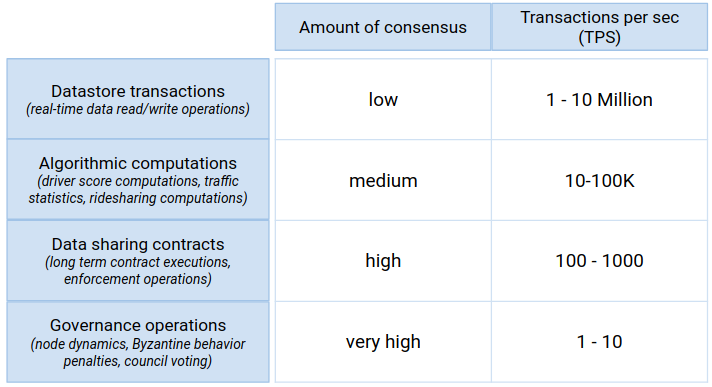
\includegraphics[width=0.75\textwidth]{tps_lat2.png}
  \caption{Expected Transaction per second velocity of various types of functionalities on the Latitude Blockchain.}
    \label{fig:tps_lat}
\end{figure}

